% ==================== 三、软件架构设计 ====================
\section{软件架构设计}

\subsection{为什么是「分层 + 领域模块化」}

实验一的需求里，真正难的从来不是「把界面做出来」，而是三件会互相打架的事：库存不能被两个人同时卖出、改价不能和下单撞在半个价格上、订单与房间两个状态机必须同步推进。这三件事的共同点是——\textbf{它们都要求某个最小粒度的东西只有一个权威副本}。库存的权威副本是「房型 $\times$ 日期」这一格，价格的权威副本也是这一格，订单状态的权威副本是订单表的 `status` 列。

由此推出架构的第一条约束：\textbf{任何可能被并发写入的业务概念，只能有一个存储点、一种写入口}。这条约束直接决定了系统长成「单体应用 + 一个 MySQL」，而不是微服务。

第二条约束来自角色：四个端面对的界面完全不同，但它们操作的是同一批业务对象。如果把「顾客端下单」和「前台线下开单」写成两套扣库存逻辑，两边迟早会对不上，超卖只是时间问题。因此表现层可以分裂成四套，\textbf{领域层必须合并成一套}。

两条约束合起来，就是本设计采用的架构风格：\textbf{按层分离部署形态，按领域划业务模块，模块之间单向依赖，事件解耦环}。

\subsection{分层与包结构}

图 \ref{fig:pkg} 是包图。四层从上到下依次是表现层、接入层、领域层、基础设施层，依赖方向严格向下，不允许反向。

\begin{figure}[htbp]
\centering
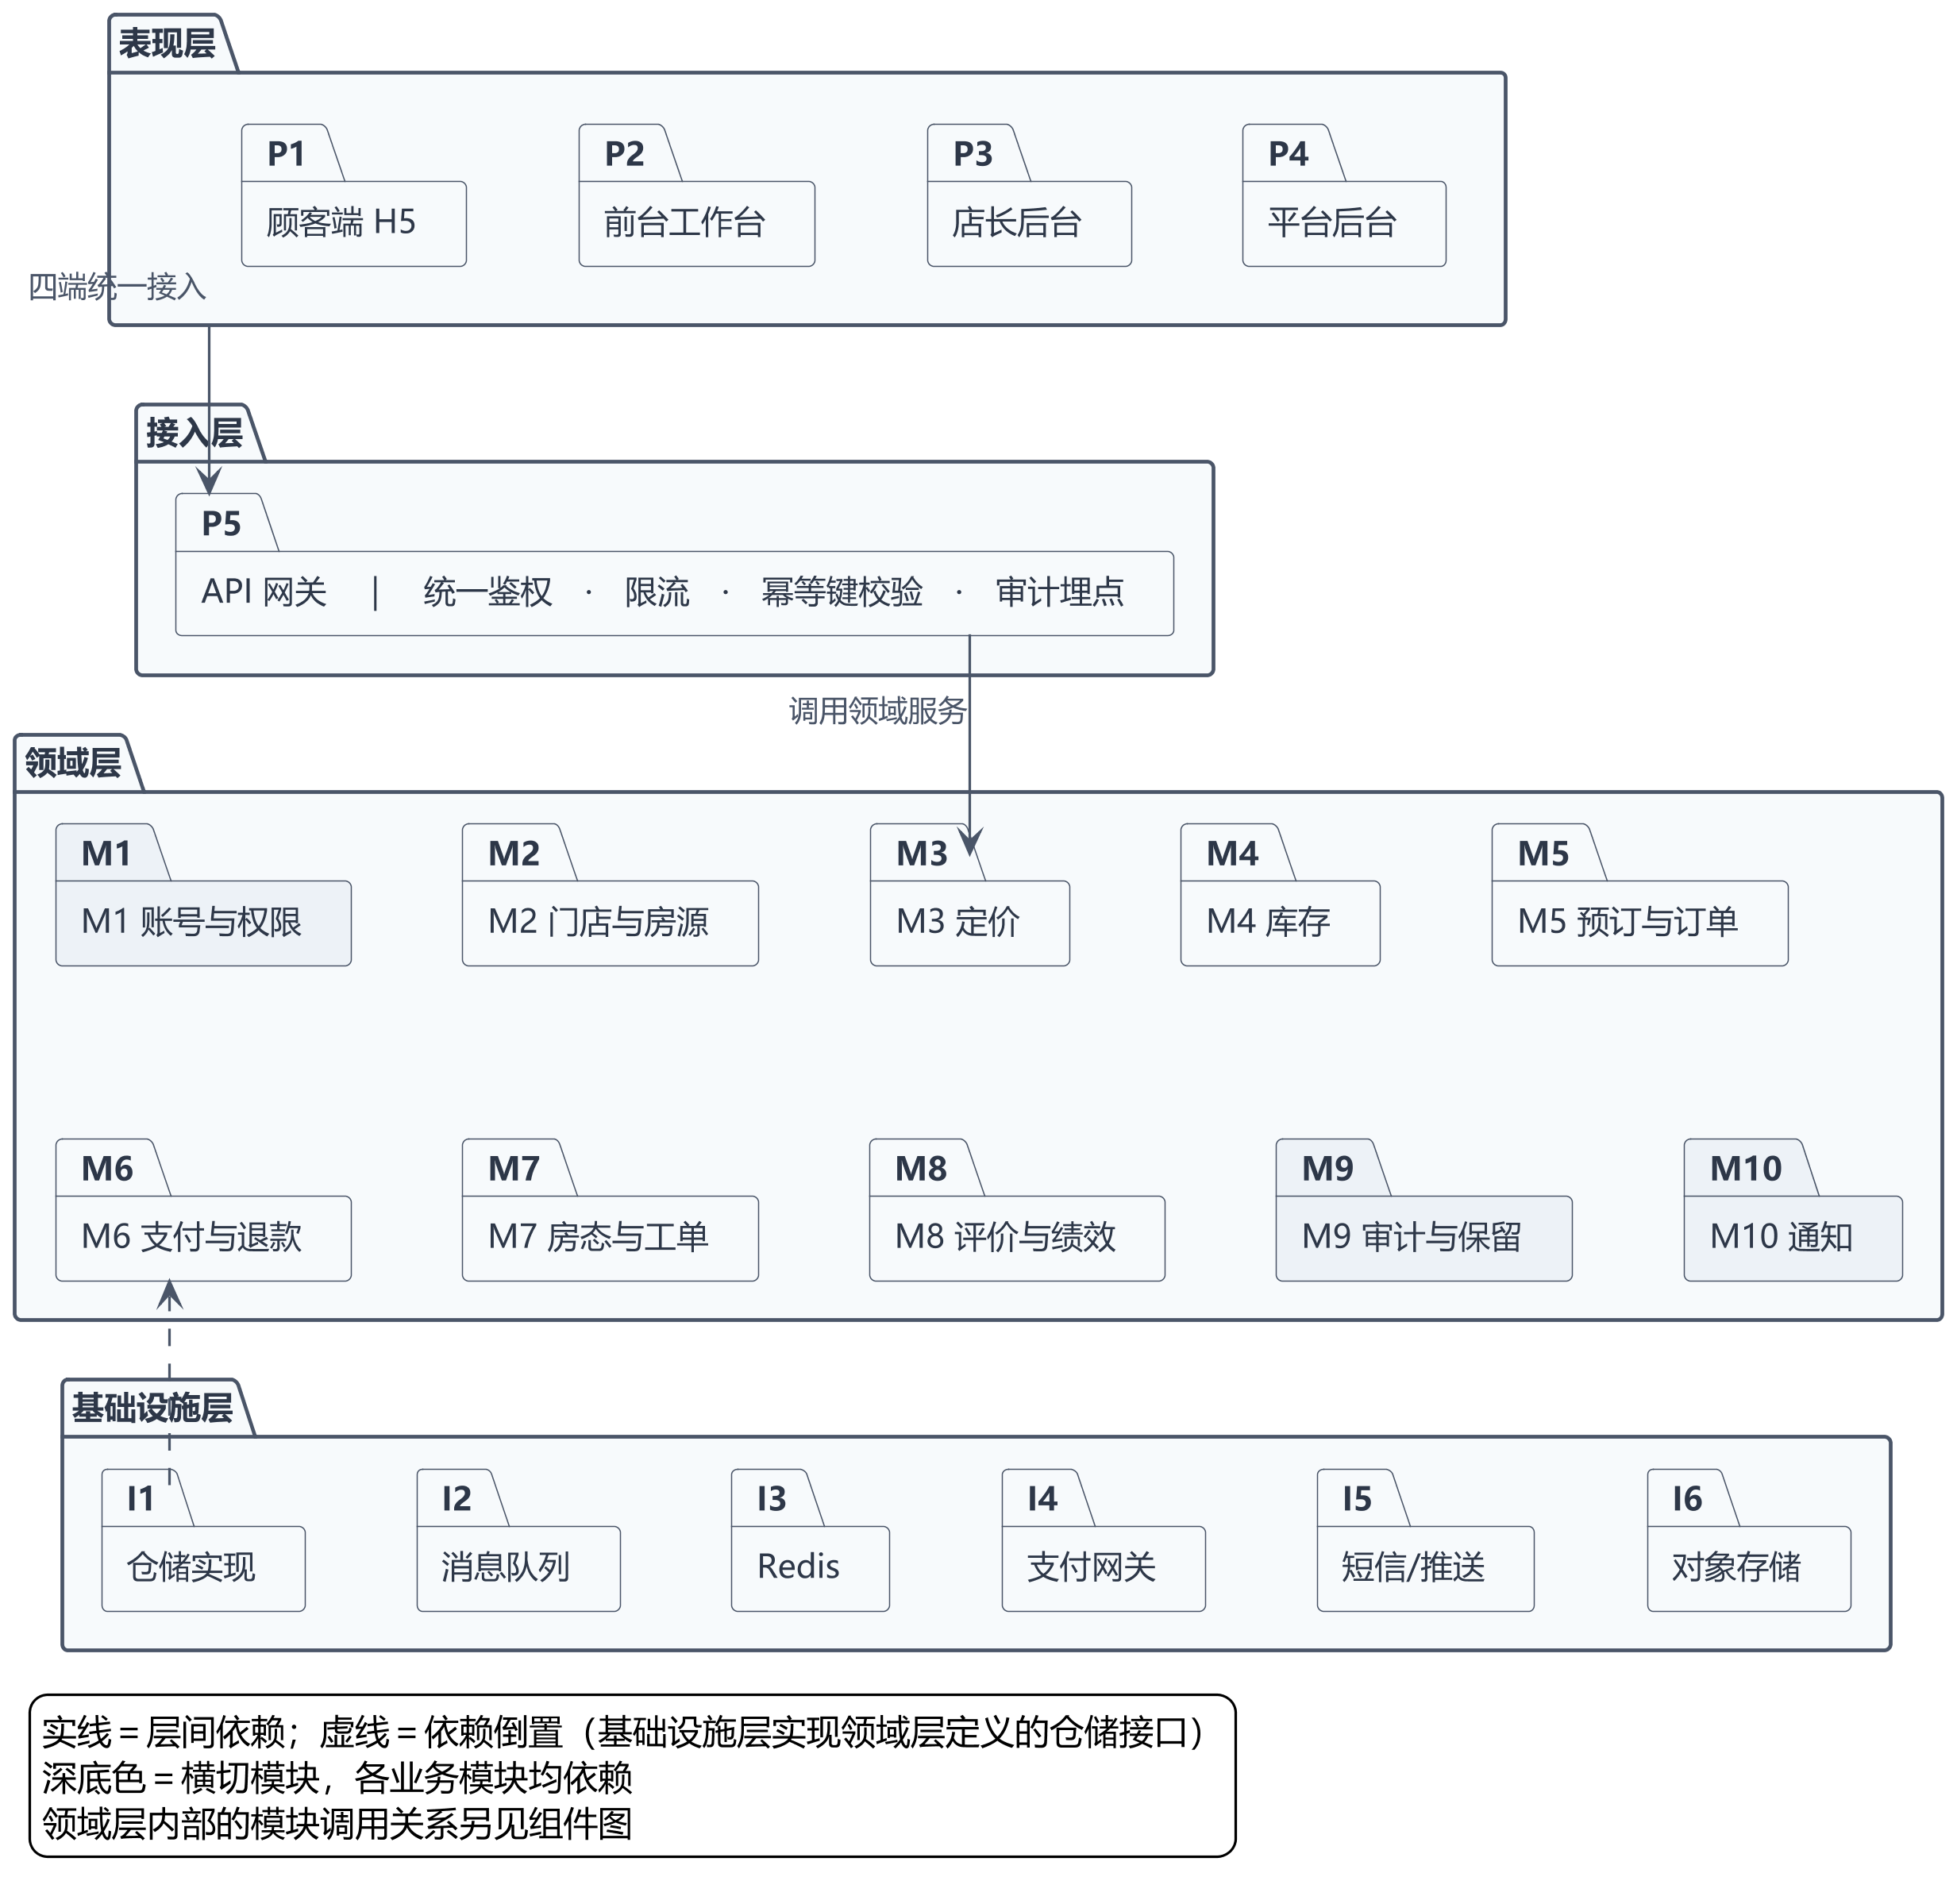
\includegraphics[width=0.96\textwidth]{../UML/UML包图.png}
\caption{UML 包图：四层结构与十个领域包}
\label{fig:pkg}
\end{figure}

四个层的职责与被禁止的动作：

\begin{itemize}
  \item \textbf{表现层}：四个独立前端，只做渲染与表单校验。不允许把业务规则写在前端——REQ-027 明确要求服务端独立校验，前端的校验只是体验，不是保障。
  \item \textbf{接入层}：API 网关，做鉴权、限流、幂等键校验、审计埋点。它是唯一知道「谁在调用」的地方，因此也是最省事的越权拦截点。
  \item \textbf{领域层}：十个模块，全部业务规则在这里。领域层\textbf{不认识} HTTP，也不认识具体数据库——它依赖的是仓储接口。
  \item \textbf{基础设施层}：仓储实现、消息队列、Redis、支付网关适配、短信适配、对象存储。它实现领域层定义的接口，箭头是\textbf{反向的虚线}（依赖倒置）：不是领域层去 new 一个 MySQL，而是基础设施层去实现它。
\end{itemize}

包图里有一条不太显眼但很关键的约束：\textbf{领域层内部没有跨越层的捷径}。例如 M5 想释放库存，必须走 M4 的接口，不能直接更新 `日库存` 表。这条约束看起来啰嗦，但它保证了「库存只有 M4 会改」——一旦允许绕过，REQ-011 的并发正确性就失去了推理基础。

\subsection{模块划分与依赖关系}

\subsubsection{组件图读法}

图 \ref{fig:comp} 是组件图。实线是调用依赖，虚线是事件订阅，方向即依赖方向。

\begin{figure}[htbp]
\centering
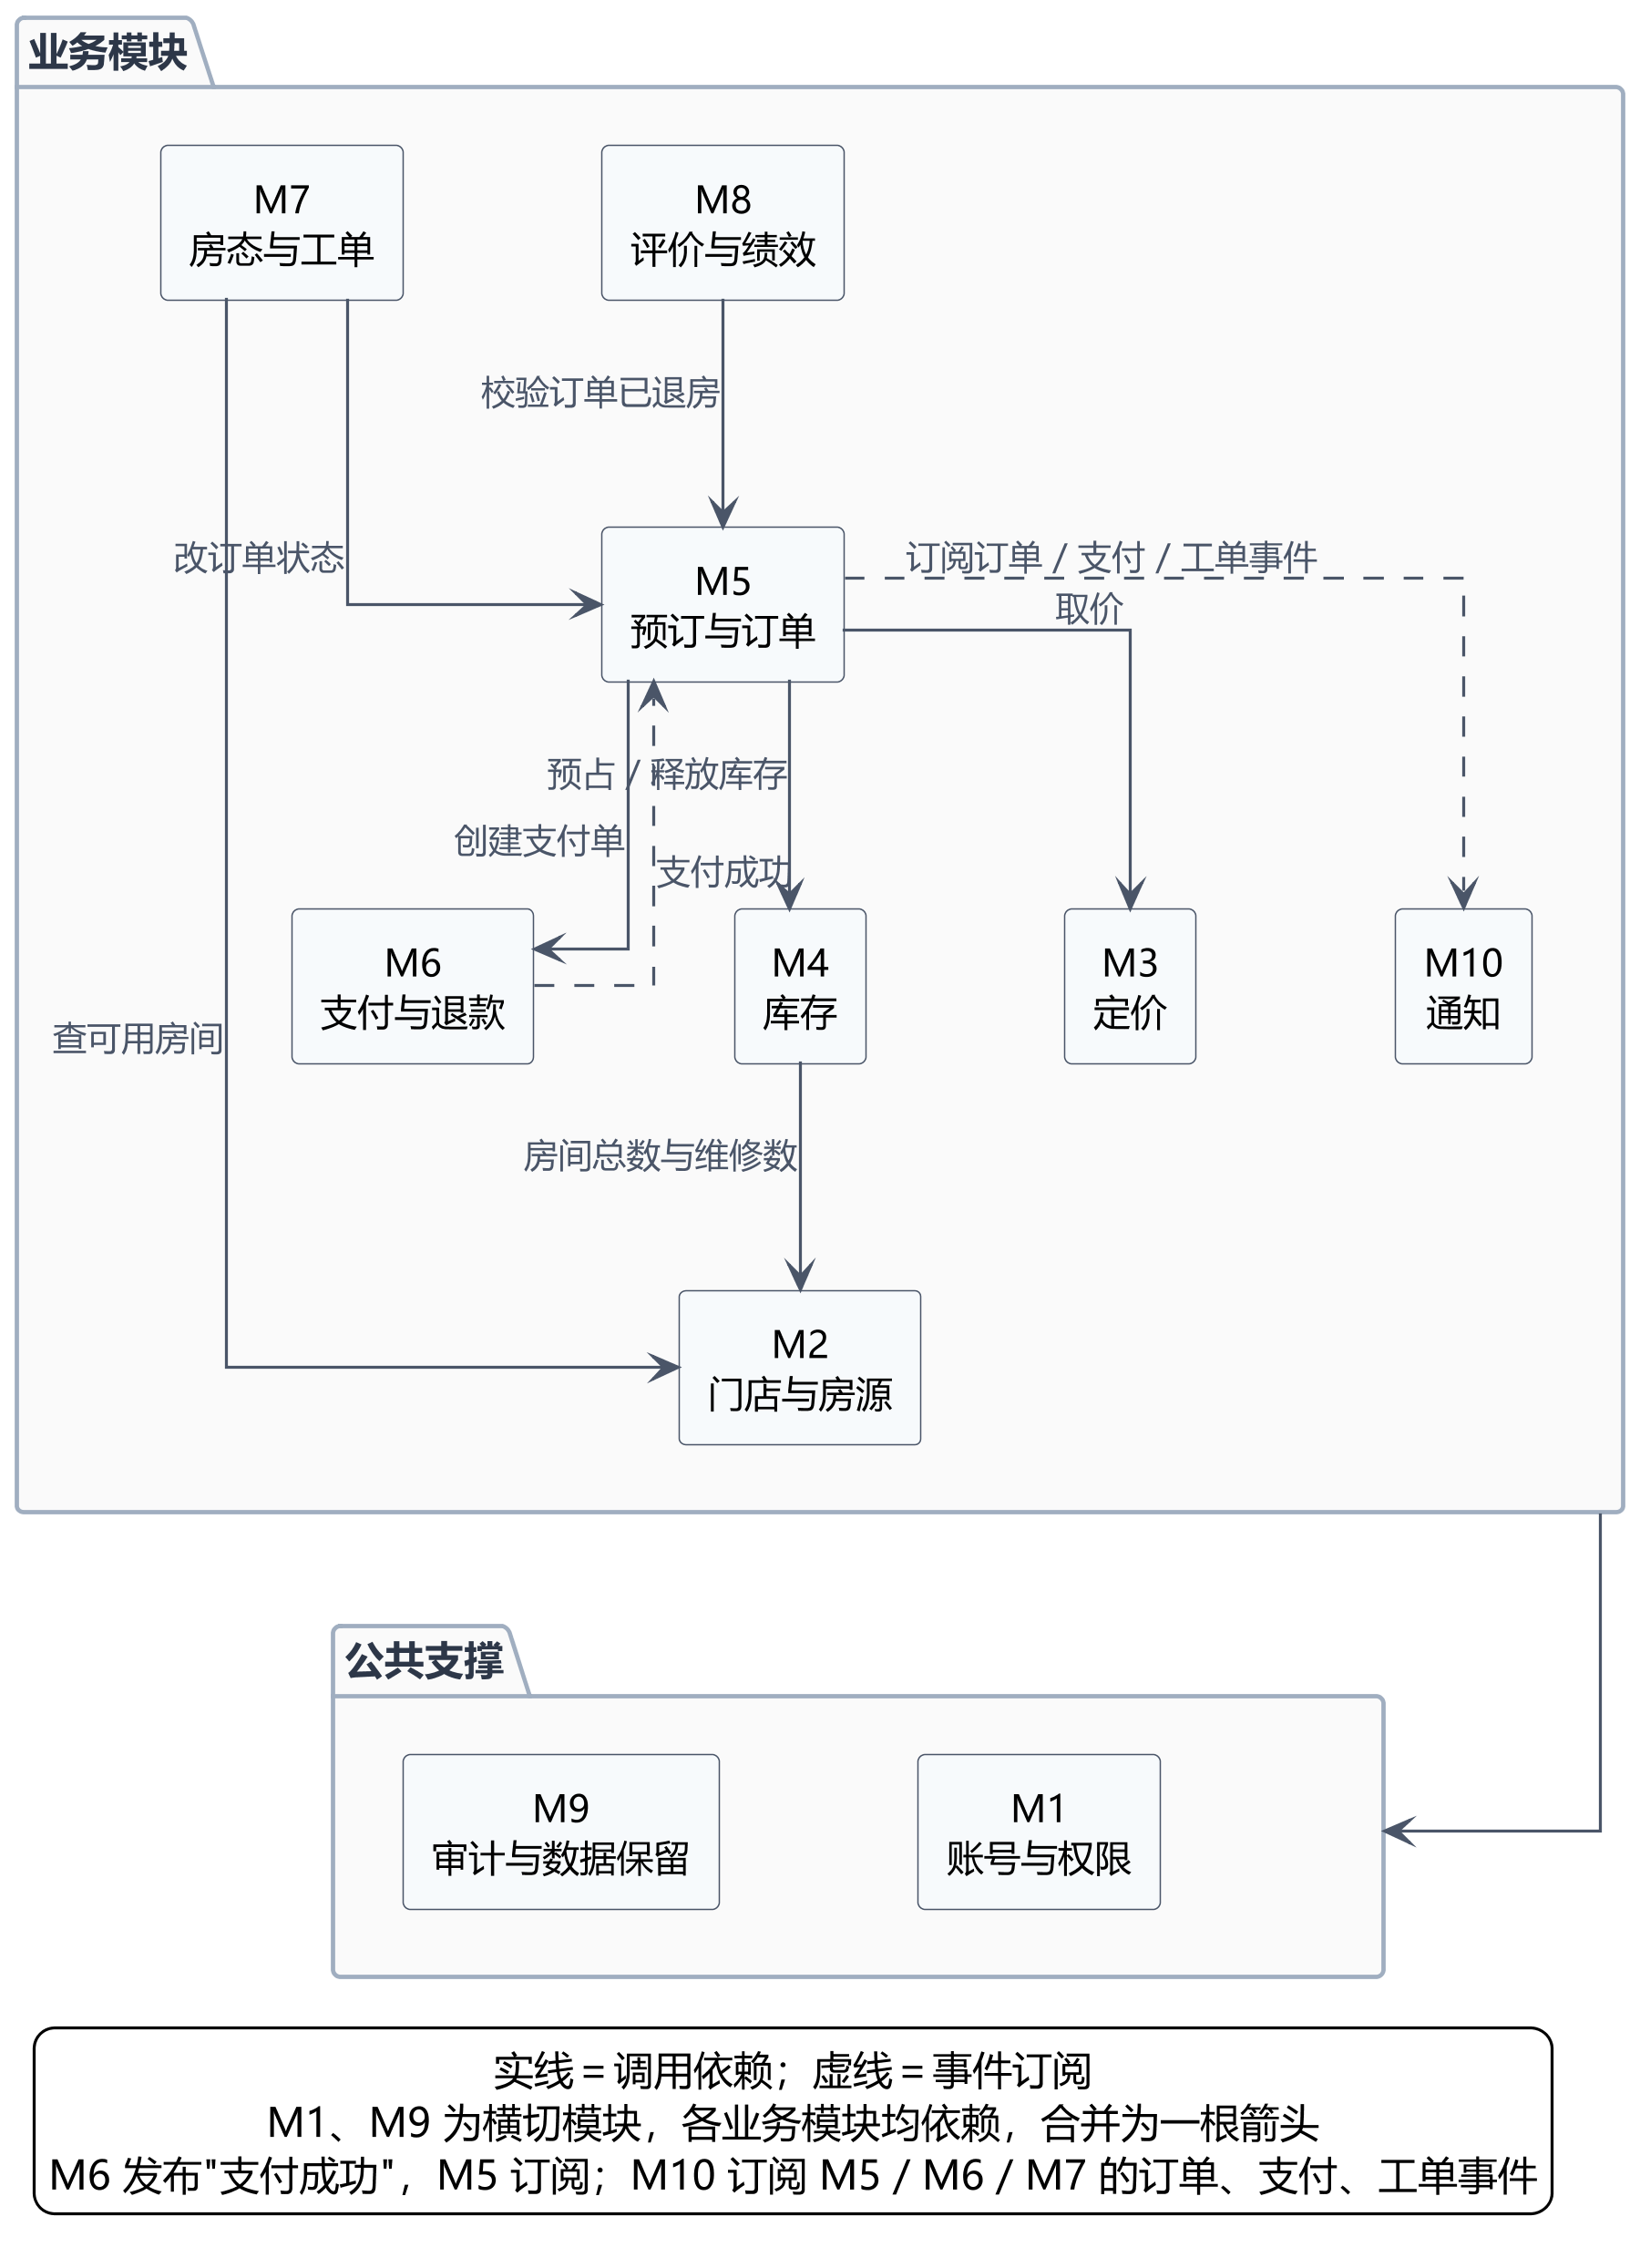
\includegraphics[width=0.68\textwidth]{../UML/UML组件图.png}
\caption{UML 组件图：十个模块的调用依赖与事件订阅}
\label{fig:comp}
\end{figure}

图上有\textbf{九条}依赖，逐条都有对应的业务事实：

\begin{table}[H]
\centering
\caption{组件图上的依赖及其依据}
\tabfont
\begin{tabularx}{\textwidth}{@{}L{2.5cm}L{1.8cm}X@{}}
\toprule
依赖 & 类型 & 为什么存在 \\
\midrule
M5 $\rightarrow$ M4 & 调用 & 下单预占、取消与超时释放库存（REQ-011、REQ-013） \\
M5 $\rightarrow$ M3 & 调用 & 下单取价并生成价格快照（REQ-023） \\
M5 $\rightarrow$ M6 & 调用 & 用户点「去支付」时创建支付单（不在下单时创建，见决策四） \\
M6 $\rightarrow$ M5 & 事件 & 支付成功后 M6 只发事件，M5 订阅后自行推进订单状态 \\
M4 $\rightarrow$ M2 & 调用 & 计算可售上限需要房间总数与维修间数（REQ-033、REQ-034） \\
M7 $\rightarrow$ M2 & 调用 & 排房时查询可用房间（REQ-024） \\
M7 $\rightarrow$ M5 & 调用 & 入住与退房要同步推进订单状态（REQ-004） \\
M8 $\rightarrow$ M5 & 调用 & 提交评价前校验订单已退房（REQ-003） \\
M5、M6、M7 $\rightarrow$ M10 & 事件 & 订单、支付、工单事件触发通知（REQ-029） \\
\bottomrule
\end{tabularx}
\end{table}

\subsubsection{三处边界约定的理由}

模块划分最容易被质疑的不是「切成了几块」，而是「某个职责为什么放在这块」。本设计有三处是讨论后才定的，都写在这里：

\textbf{一、维修标记放在 M2 的房间档案上，M7 只是改它的入口。} 库存要算可售上限，必须拿到「这间房在哪些日期维修」，而库存不能反过来依赖房态模块——那会让库存回算路径变成 M4 $\rightarrow$ M7 $\rightarrow$ M2 三段。把维修日期作为房间档案的一个字段，M4 只需要依赖 M2 一段。代价是 M7 改房态时写的是 M2 的表，看起来越界，但这是有意为之的取舍。

\textbf{二、排房归 M7，不归 M2。} M2 只管「这栋楼有几间房、几间在修」，是静态档案；「今天这间房被哪张订单占着」是动态事实，属于房态。若把排房交给 M2，M2 就要持有占房记录并维护唯一性，而它原本是无状态的档案模块。

\textbf{三、M10 只订阅事件，绝不反向调用业务模块。} 这条约束的意思是：事件载荷里必须带够渲染通知所需的字段（订单号、金额、顾客联系方式、时间），M10 不能回头查 M5 补全。不守住这条，实验三实现时一定会退化成「M10 调 M5 查订单」，于是通知模块一旦故障就会拖慢下单。

\subsubsection{横切模块的画法}

M1 账号与权限、M9 审计与数据保留被所有业务模块依赖。组件图上没有画十根箭头——那样图会被压成一张蜘蛛网，反而看不出业务模块之间的关系。折中的画法是把两者放进「公共支撑」带，各业务模块汇一根箭头指过去。

这里需要说明的是：\textbf{这个折中本身是违反「画全」原则的}，因为 M1、M9 在图上的连线不完整。做出这个选择的原因是作业要求「写明软件的模块划分」，一张看不出结构的完整图等于没画；而缺失的那部分信息在上表与本节文字里已经补齐。

\subsection{模块之间的交互}

组件图只说了「谁依赖谁」，没说「什么时候、按什么顺序」。这要靠时序图与活动图（图 \ref{fig:seq1}--\ref{fig:act2}，说明见 5.4 节）。这里先概括三处最关键的交互：

\subsubsection{下单与扣库存}

顾客提交订单时携带请求号，网关按请求号做幂等校验，M5 在同一事务内完成「条件扣减库存 + 插入待支付订单」。库存扣减写在 SQL 的 WHERE 子句里：

\begin{quote}
\zihao{5}\ttfamily
UPDATE inventory SET sold = sold + n\\
WHERE room\_type = ? AND stay\_date = ? AND sold + n <= online\_limit
\end{quote}

影响 0 行就是抢房失败，不需要「先查再改」。这不是性能优化，而是正确性要求：先查再改之间只要有间隙，100 并发下必然超卖（REQ-011、REQ-015）。

\subsubsection{支付回调与订单生效}

支付平台异步回调时，M6 依次做三件事：验签、按支付单号判重、按订单\textbf{此刻}的状态决定落点。状态是待支付就转已确认并保留库存；状态已被超时任务改成已取消，就不再恢复订单——库存可能已经被别人买走——而是发起原路退款。这条分支是 REQ-028「不得出现已扣款而无对应订单」的具体实现。

\subsubsection{改价与下单互斥}

店长改价与顾客下单在同一格「房型 $\times$ 日期」上互斥，锁的范围只覆盖「读旧价 $\rightarrow$ 写新价 $\rightarrow$ 提交」这一小段，毫秒级。等锁超过 300 ms 就返回重试提示，\textbf{不允许静默使用旧价}——静默用旧价等于把一次改价悄悄吞掉。

\subsection{部署形态}

\begin{figure}[htbp]
\centering
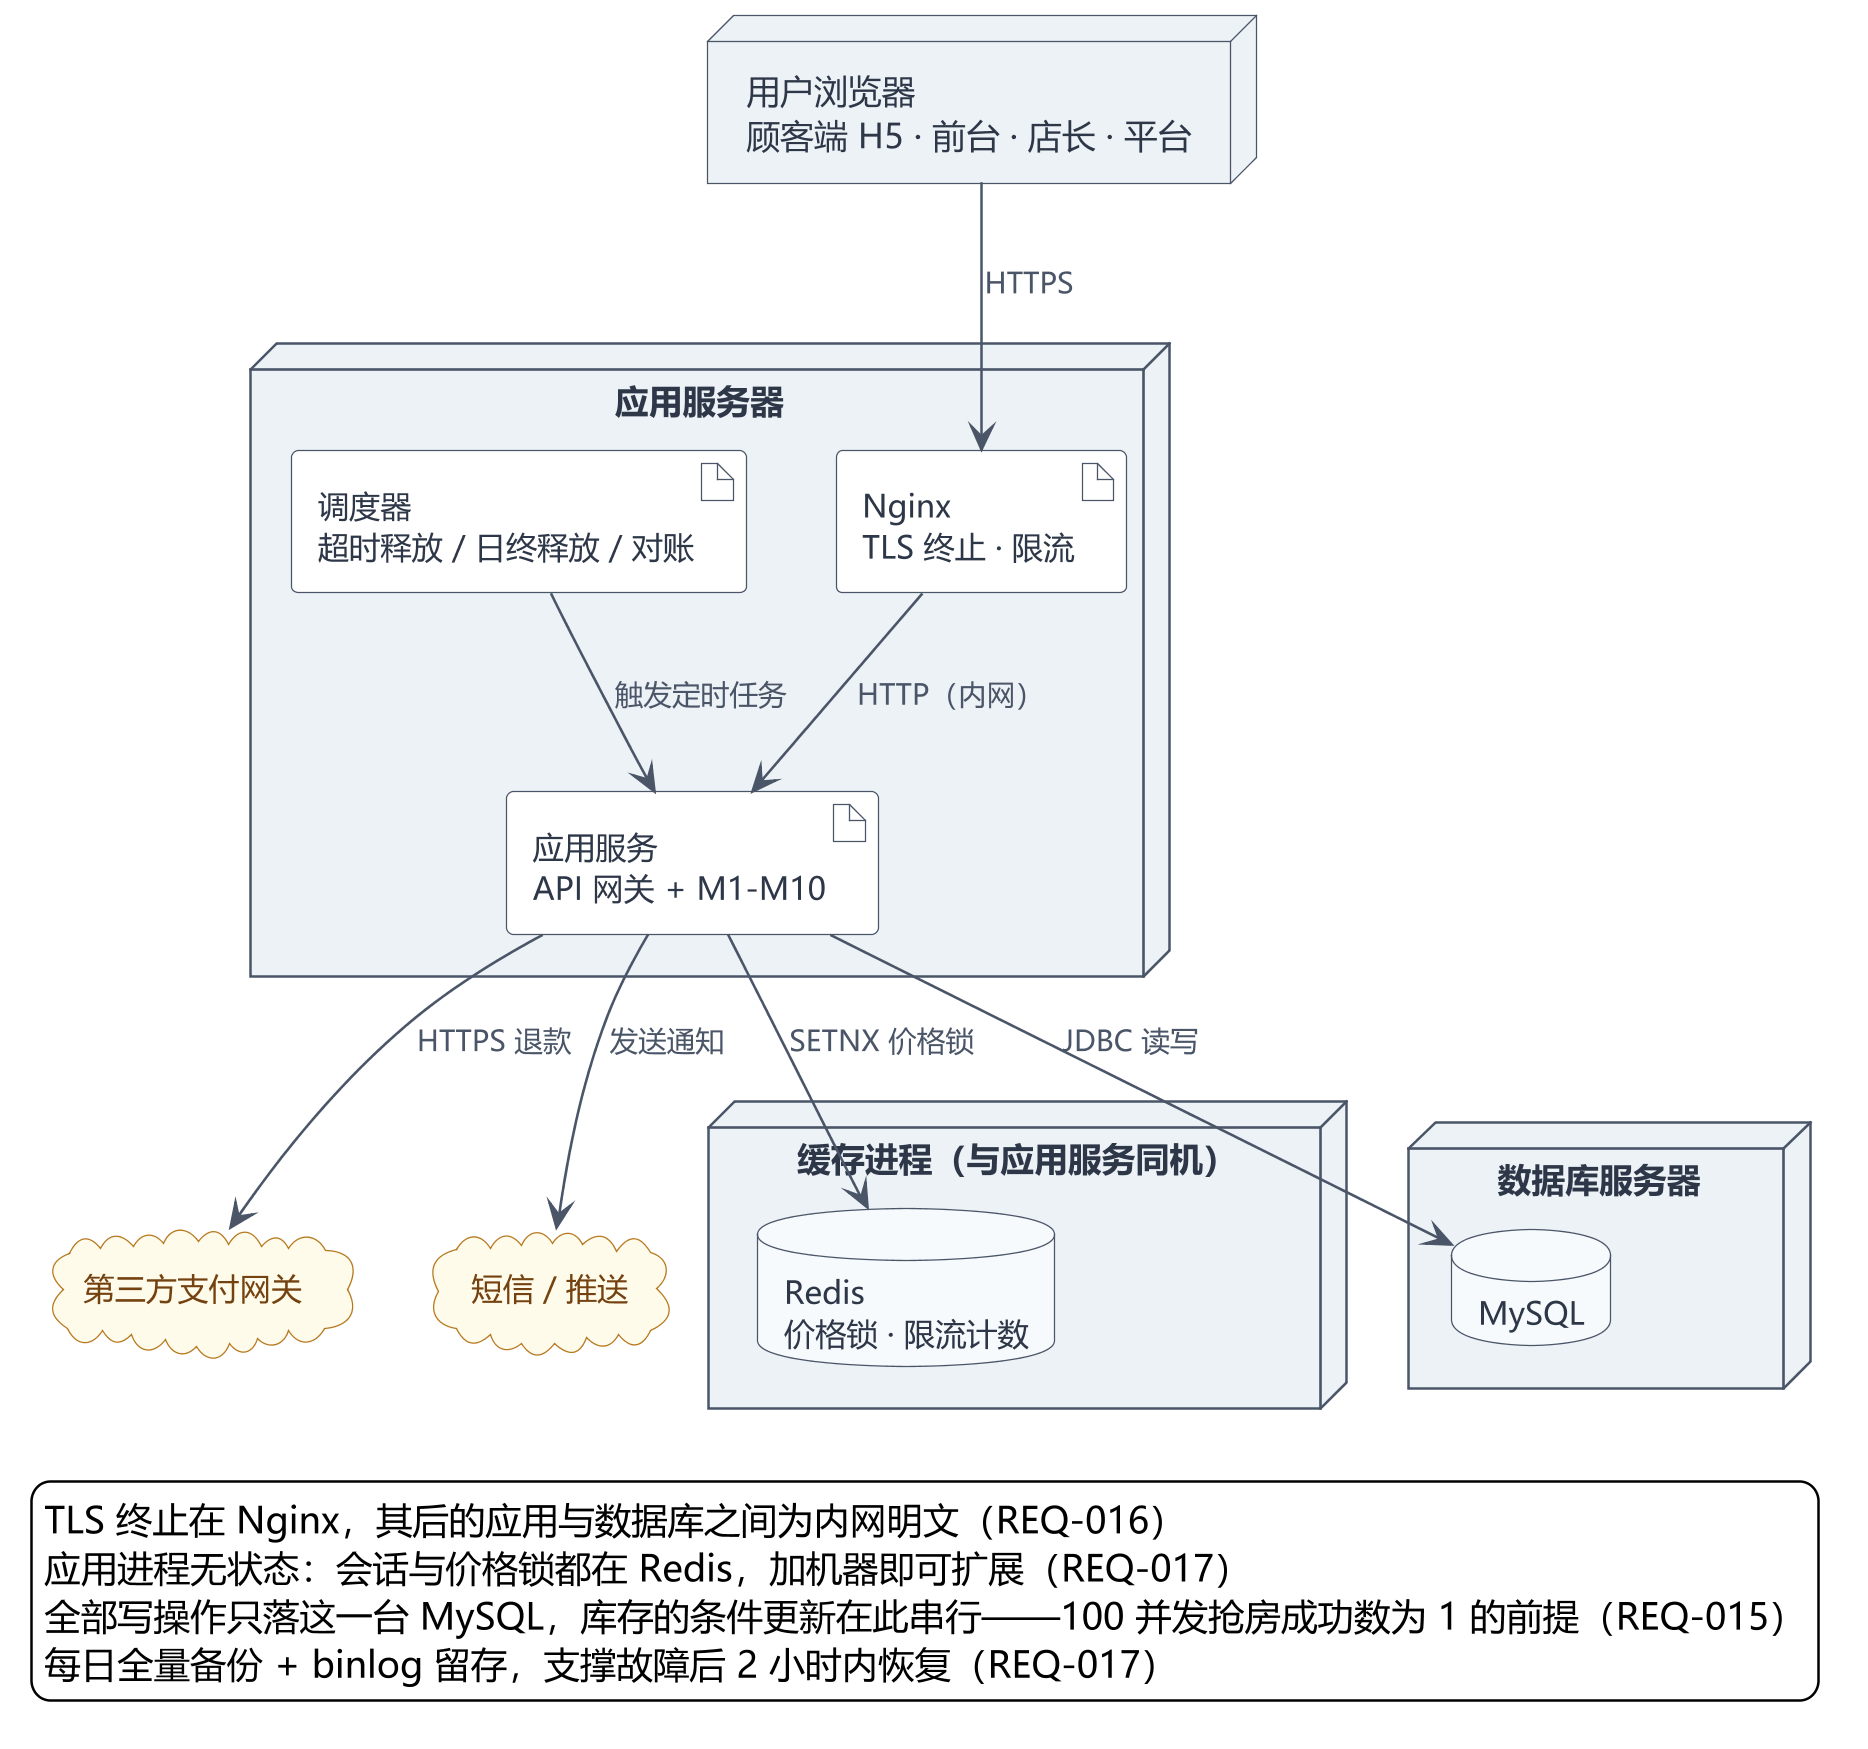
\includegraphics[width=0.92\textwidth]{../UML/UML部署图.png}
\caption{UML 部署图：应用、缓存、数据库与三类外部系统}
\label{fig:deploy}
\end{figure}

图 \ref{fig:deploy} 是部署图，四个要点：

\begin{itemize}
  \item \textbf{TLS 终止在 Nginx}，其后应用与数据库之间为内网明文。这不是省事，而是内网段本身不对外，再做一层 TLS 只会增加证书轮换成本（REQ-016 只要求「全站通过 HTTPS 传输」，指的是用户侧）。
  \item \textbf{应用进程无状态}：会话与价格锁都在 Redis，加机器即可扩展。这意味着可以横向加应用节点，但\textbf{不能}横向加数据库——库存的条件更新必须在同一台 MySQL 上串行，这是 100 并发抢房成功数为 1 的前提。
  \item \textbf{调度器与应用同机部署}，负责支付超时扫描、日终保留释放、每日对账。选同机是因为它只是一个定时触发循环，拆成独立进程反而要多一套部署与监控。
  \item \textbf{唯一写库}：去掉主从读写分离对写的影响，读请求可以走从库，写请求全部落主库。
\end{itemize}

\subsection{八条关键设计决策与代价}

架构设计最容易被问的问题是「为什么不那样做」。下面八条是本设计里争议最大、也最需要说清代价的取舍。

{\tabfont
\begin{xltabular}{\textwidth}{@{}p{0.5cm}p{3.3cm}X@{}}
\caption{关键设计决策与代价}\label{tab:decisions}\\
\toprule
\# & 决策 & 取舍与代价 \\
\midrule
\endfirsthead
\toprule
\# & 决策 & 取舍与代价 \\
\midrule
\endhead
\midrule
\multicolumn{3}{r}{\zihao{6}续下页}\\
\endfoot
\bottomrule
\endlastfoot
一 & 单体应用而非微服务 & 换来「扣库存 + 落单」是一个本地事务，不超卖可以只靠数据库保证。代价是模块只能靠代码边界约束，不能靠进程隔离；某个模块内存泄漏会拖垮全站。以本系统的量级（日均百单、十余间房），这个代价可以接受。 \\
二 & 库存记在「房型 $\times$ 日期」而非房间上 & 下单时顾客并不知道住哪间，REQ-024 也是「先占房型、入住前才排房」。代价是查询余量要按日期范围聚合，且排房时需要另一次「房间是否被占」的判定——这个判定落在 M7 的占房记录上。 \\
三 & 库存只信 MySQL 行锁，Redis 不承担计数 & 换来不存在「缓存与数据库双写不一致」这一类问题，REQ-017 的数据一致性有单点可依。代价是并发高峰时库存这一行会成为热点行，吞吐受限；本系统的峰值并发是 100 个请求抢 1 间房，MySQL 足够。 \\
四 & 支付单在「去支付」时创建，不在下单时创建 & 换来支付网关故障不波及下单——网关挂了，顾客仍能正常下单，只是暂时付不了款。代价是订单与支付单不是同时产生的，对账时可能出现「订单存在但无支付单」的正常中间态，判断差异时必须排除超时未支付这一种。 \\
五 & 订单与房间各一台状态机，转换表驱动 & 换来非法转换有唯一处理方式（抛异常并提示当前实际状态），而不是各处的 if-else 各写各的。代价是每次新增状态都要同时改三处：状态枚举、转换表、界面文案，漏一处就会在某个入口上崩。 \\
六 & 订单明细存价格快照 & 换来改价不影响历史订单（REQ-023），退款金额也有据可查。代价是订单表与价格表之间多一份冗余，出现「同一晚两个价格」时必须能解释清楚哪一个是快照、哪一个是当前价——界面上不展示当日价时不标「当前价」就是错的。 \\
七 & 查询走缓存，写一律落主库 & REQ-015 要求 50 并发下查询 2 秒内返回。房型与价格是读多写少，加一层本地缓存即可满足；写请求不缓存，避免为了刷新缓存引入一致性窗口。代价是改价后最多有一个缓存 TTL 的延迟，本设计把 TTL 设为 5 秒，并在改价成功后主动失效该房型当日的缓存条目。 \\
八 & 鉴权在网关一次做完，领域模块不重复鉴权 & 换来权限规则只有一处，改一次全站生效（REQ-016）。代价是领域模块被内部服务直接调用时没有防线，因此约定：领域模块的接口\textbf{只能}由网关或本进程内的上游模块调用，不对外开放端口。 \\
\end{xltabular}
}
